\subsection{Interpretability}
\label{sec:res-interp}

\paragraph{The contributions are exact SHAP values.} Kernel SHAP with every one of the \V{shap.coalitions} feature coalitions, a background of \V{shap.background} training tasks and \V{shap.tasks} test tasks returns the centred \kaam{} contributions of the canonical model to within \V{shap.maxdiff} log-odds, and the ten contributions plus the bias reproduce the model's logit to within \V{shap.sumgap}. No sampling enters a \kaam{} explanation; the same holds for any additive model, the additive EBM included, so this property does not favour the KAN parameterisation over other additive models.

\paragraph{The curves.} Figure~\ref{fig:curves} shows the ten curves of the canonical model for its five seeds, with the corresponding curve of the original sample. The five seeds give nearly identical curves. Validation chose no smoothness penalty on all five random splits of the full trace, and the strongest value, \V{model.lambdamax}, on the time-ordered split and on \V{full.lambda.grouped.em2} of the five user-grouped folds, where the validation tasks come from a later period or from other users. On the random splits the four request features therefore get curves that oscillate between the few values that occur (the ticks in Figure~\ref{fig:curves}); such a curve is informative only at observed values. The telemetry curves are smooth: risk rises with the recent kernel CPU of the machine and falls steeply as its recent load rises from low values, the pattern the first version reported and attributed, tentatively, to the trace recording telemetry mostly for workers that finished.

\begin{figure*}[t]
\centering
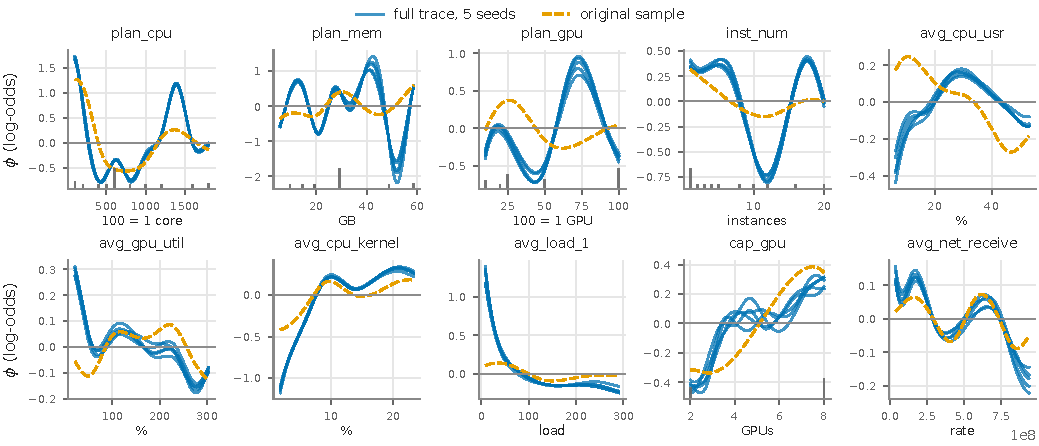
\includegraphics[width=\textwidth]{figures/curves_all.pdf}
\caption{The ten curves of the canonical \kaam{} (full trace, random split \V{prot.canon}) for five seeds, and the curve learned on the original sample (dashed), each centred on its mean over the training 5th to 95th percentile. Ticks: values of the discrete features held by at least \V{fig.tickshare} of training tasks, with height proportional to their share.}
\label{fig:curves}
\end{figure*}

\paragraph{\kaam{} against the additive EBM.} The two additive models fit their shape functions in different ways, B-splines by gradient descent and piecewise-constant terms by cyclic boosting, so their agreement is a check on both (Table~\ref{tab:shapecorr}, Figure~\ref{fig:shapes}). On the grid fixed in the protocol the median correlation over the ten features is \V{ebm.r.median}; the telemetry curves agree closely, while two request features show almost no agreement (lowest: \V{ebm.r.worstfeat}, $r=\V{ebm.r.min}$). Evaluated at the training tasks' own values, an exploratory measure not fixed in the protocol, the median correlation is \V{ebm.rd.median} and the lowest \V{ebm.rd.min} (\V{ebm.rd.worstfeat}). The disagreement is therefore concentrated between observed values of the discrete requests, where neither model has data. On the canonical split the additive EBM, fitted once on the full trace, reaches a test AUC of \V{full.s42.ebm.auc} against \V{full.s42.kaam.auc} for \kaam{}.

% Generated by scripts/paper_tables.py. Do not edit.
\begin{table}[t]
\centering
\small
\TabCaption{tab:shapecorr}{\kaam{} and additive EBM shape functions}{$r_{\mathrm{grid}}$: Pearson correlation of the two centred curves on 200 evenly spaced points between the training 5th and 95th percentiles, as fixed in the protocol. $r_{\mathrm{data}}$ (exploratory): the same correlation at the values of up to \V{ebm.rd.ntasks} training tasks inside that window, so that each value counts as often as it occurs; for the request features, which take few distinct values, the grid version mostly compares how the two models fill the gaps between observed values. Swing: maximum minus minimum of each curve over the window, in log-odds. Canonical random split of the \V{ebm.shapeds}, seed~0.}
\begin{tabular}{@{}lcccc@{}}
\toprule
Feature & $r_{\mathrm{grid}}$ & $r_{\mathrm{data}}$ & \kaam{} swing & EBM swing \\
\midrule
\feat{plan_mem} & 0.04 & 0.75 & 3.16 & 2.97 \\
\feat{plan_cpu} & 0.62 & 0.99 & 2.50 & 2.62 \\
\feat{plan_gpu} & 0.04 & 0.57 & 1.66 & 0.97 \\
\feat{avg_load_1} & 0.97 & 0.97 & 1.61 & 1.79 \\
\feat{avg_cpu_kernel} & 0.98 & 0.99 & 1.47 & 1.71 \\
\feat{inst_num} & 0.46 & 0.81 & 1.22 & 1.17 \\
\feat{cap_gpu} & 0.70 & 1.00 & 0.76 & 0.68 \\
\feat{avg_cpu_usr} & 0.90 & 0.88 & 0.54 & 0.64 \\
\feat{avg_gpu_util} & 0.85 & 0.82 & 0.43 & 0.45 \\
\feat{avg_net_receive} & 0.80 & 0.76 & 0.29 & 0.47 \\
\bottomrule
\end{tabular}
\TabNotes
\end{table}


\begin{figure*}[t]
\centering
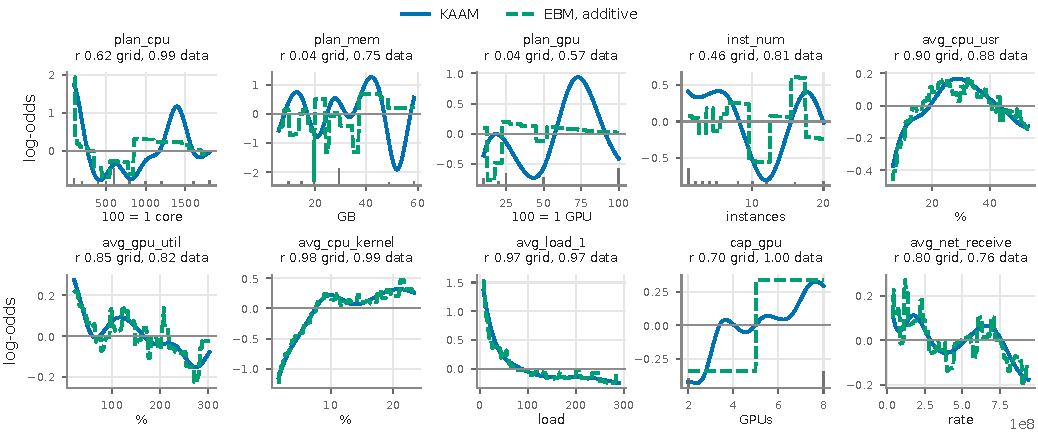
\includegraphics[width=\textwidth]{figures/shapes_kaam_ebm.pdf}
\caption{Shape functions of \kaam{} and of the additive EBM on the canonical split, centred on their means over the training 5th to 95th percentile. Panel titles give the correlation on the protocol's evenly spaced grid and at the training tasks' values. Ticks as in Figure~\ref{fig:curves}.}
\label{fig:shapes}
\end{figure*}

\paragraph{The one-core curve under each protocol.} Figure~\ref{fig:plancpu} overlays the \feat{plan_cpu} curve of the first seed under every protocol of the full trace. On the canonical split the centred curve stands at \V{pc.randoms42.onecore} log-odds at one core. With User~1 removed it stands at \V{pc.louod1.onecore}, and with Users~1 and~4 removed at \V{pc.louod14.onecore}. In the user-grouped folds the value at one core ranges from \V{pc.grouped.minone} to \V{pc.grouped.maxone}; the lowest is fold~\V{full.mech.u1fold}, whose training set also lacks User~1. A centred value reflects the whole shape of a curve as well as the one-core effect, and the shape changes from fit to fit (correlation with the canonical curve between \V{pc.groupedf1.corr} and \V{pc.groupedf0.corr} over the grouped folds, \V{pc.timet.corr} for the time-ordered split), so the training data give the clearer evidence: with User~1 in training, one-core tasks fail at \V{rf.oc.with.minone} to \V{rf.oc.with.maxone} against \V{rf.oc.with.minother} to \V{rf.oc.with.maxother} for other tasks, and without User~1 at \V{rf.oc.groupedf4.one} against \V{rf.oc.groupedf4.other} (fold~\V{full.mech.u1fold}) and \V{rf.oc.louod1.one} against \V{rf.oc.louod1.other} (split without User~1). Centring on the mean training task instead of the grid, a post hoc check, a one-core request adds \V{ph.oc.randoms42} log-odds on the canonical split and \V{ph.oc.gwith.min} to \V{ph.oc.gwith.max} in the grouped folds whose training users include User~1, against \V{ph.oc.louod1} without User~1 and \V{ph.oc.louod14} without Users~1 and~4. Fold~\V{full.mech.u1fold}, trained without User~1, still gives \V{ph.oc.gwithout}, although its one-core and other training tasks fail at \V{ph.oc.gwithout.trone} and \V{ph.oc.gwithout.trother}. The curves are a complete account of each fitted model; they are not a stable account of the data. A second rise near thirteen cores appears with and without User~1 but not in the time-ordered curve.

\begin{figure}[t]
\centering
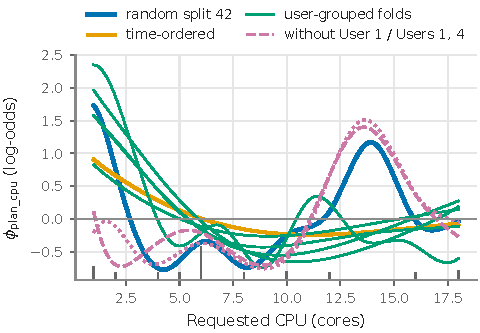
\includegraphics[width=0.62\linewidth]{figures/plan_cpu_protocols.pdf}
\caption{The \feat{plan_cpu} curve of \kaam{} (first seed) under each protocol of the full trace, centred on the same window. Ticks: request values held by at least \V{fig.tickshare} of the canonical training tasks.}
\label{fig:plancpu}
\end{figure}

\subsection{Case audits}
\label{sec:res-cases}

The four cases were selected on the canonical model's test set by the rule fixed in the first version: the most confident true positive and true negative, and the false negative and false positive with the highest risk at a threshold of 0.5 (Table~\ref{tab:cases}, Figure~\ref{fig:waterfall}). Each bar is the contribution of one feature relative to the mean training task, whose logit is \V{case.baselogit}; in every case the ten contributions and the bias reproduce the logit to within \V{case.maxsumgap}.

The true positive (risk \V{case.tp.risk}) is a one-core request, and \feat{plan_cpu} contributes \V{case.tp.c.plancpu}, \V{case.tp.topshare} of the total absolute push. The identical four-field request occurs in \V{case.tp.samereq} training tasks, \V{case.tp.samerate} of which failed and \V{case.tp.sameu1} of which came from User~1. The false positive (risk \V{case.fp.risk}) is also a one-core request and receives the same \V{case.fp.c.plancpu} from \feat{plan_cpu}, plus \V{case.fp.c.planmem} from a large memory request. Its own request occurs in only \V{case.fp.samereq} training tasks, \V{case.fp.samerate} of which failed and none from User~1: the one-core term learned largely from one user's recurring job is applied to another user's task. The false negative (risk \V{case.fn.risk}, just below the threshold) requests half a core (\V{case.fn.c.plancpu}) and \V{case.fn.raw.instnum} instances (\V{case.fn.c.instnum}); its request occurs in \V{case.fn.samereq} training tasks with a failure rate of \V{case.fn.samerate}. The true negative (risk \V{case.tn.risk}) owes most of its score to \feat{plan_gpu} at the \V{case.tn.pct.plangpu} percentile (\V{case.tn.c.plangpu}); its exact request occurs in \V{case.tn.samereq} training tasks, none of which failed. A confident score that rests on a sparse region of one feature is visible at a glance in this form.

% Generated by scripts/paper_tables.py. Do not edit.
\begin{table*}[t]
\centering
\small
\TabCaption{tab:cases}{Four case audits of the canonical \kaam{}}{Selected by the rule fixed in advance (most confident true positive and true negative; highest-risk false negative and false positive at threshold 0.5). Contributions are log-odds relative to the mean training task. Same request: training tasks with the identical four resource requests / their failure rate / the share submitted by User~1.}
\begin{tabular}{@{}lcp{7.2cm}l@{}}
\toprule
Case & Risk & Largest three contributions & Same request \\
\midrule
True positive & 0.861 & \feat{plan_cpu} +1.68; \feat{avg_load_1} +0.41; \feat{avg_cpu_kernel} +0.36 & 44,191 / 87\% / 100\% \\
True negative & 0.002 & \feat{plan_gpu} $-$4.32; \feat{plan_cpu} $-$0.80; \feat{cap_gpu} $-$0.50 & 18 / 0\% / 0\% \\
False negative & 0.500 & \feat{plan_cpu} +1.60; \feat{inst_num} $-$0.86; \feat{cap_gpu} +0.22 & 1,995 / 5\% / 0\% \\
False positive & 0.878 & \feat{plan_cpu} +1.68; \feat{plan_mem} +0.79; \feat{avg_cpu_kernel} +0.26 & 44 / 5\% / 0\% \\
\bottomrule
\end{tabular}
\TabNotes
\end{table*}


\begin{figure*}[t]
\centering
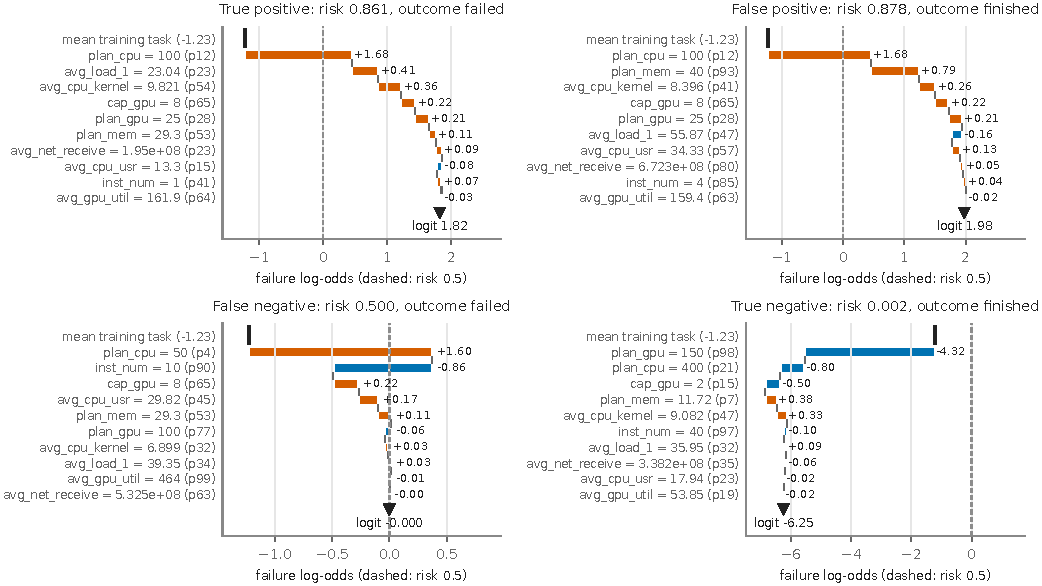
\includegraphics[width=\textwidth]{figures/case_waterfall.pdf}
\caption{Case audits of the canonical \kaam{}. Each panel runs from the logit of the mean training task (top) through the ten contributions, largest first, to the model's logit (bottom). The mean training task's logit is the bias plus each contribution's mean over training tasks. Labels give the raw value and its percentile among training tasks (pNN); the dashed line is risk 0.5.}
\label{fig:waterfall}
\end{figure*}

\subsection{Lookback window}
\label{sec:res-lookback}

On the original sample each window keeps the split roles of the one-hour build, and \kaam{} is refitted for each window (Table~\ref{tab:lookback}, Figure~\ref{fig:lookback}). On the test tasks scored at both widths, the windows of \V{lb.wide} score between \V{lb.2.diff} and \V{lb.6.diff} AUC above the one-hour model, and the half-hour window differs from it by \V{lb.0p5.diff}; after Holm correction \V{lb.nsig} of the four differences is significant, and none exceeds \V{lb.maxabsdiff}. The one-hour window is a reasonable default, and the conclusions do not depend on it.

% Generated by scripts/paper_tables.py. Do not edit.
\begin{table}[t]
\centering
\small
\setlength{\tabcolsep}{3pt}
\TabCaption{tab:lookback}{Lookback window ablation on the original sample}{Each window keeps the canonical 1\,h split roles of its tasks. Own AUC: on the window's own test set. $\Delta$: AUC minus the 1\,h model on the test tasks both score, with the paired 95\% interval; $p$ is Holm-adjusted over the four windows. \kaam{}, seed~0.}
\begin{tabular}{@{}lrrcrcc@{}}
\toprule
Window & Tasks & Test & Own AUC & Shared & $\Delta$ [95\% CI] & $p_{\mathrm{Holm}}$ \\
\midrule
0.5\,h & 17,751 & 2,671 & 0.760 & 2,671 & 0.000 [$-$0.002, 0.002] & 0.707 \\
1\,h & 18,890 & 2,834 & 0.753 & -- & reference & -- \\
2\,h & 19,524 & 2,930 & 0.753 & 2,834 & +0.003 [0.001, 0.005] & 0.032 \\
4\,h & 19,911 & 2,988 & 0.752 & 2,834 & +0.004 [0.001, 0.007] & 0.069 \\
6\,h & 20,067 & 3,011 & 0.750 & 2,834 & +0.004 [0.000, 0.008] & 0.069 \\
\bottomrule
\end{tabular}
\TabNotes
\end{table}


\begin{figure}[t]
\centering
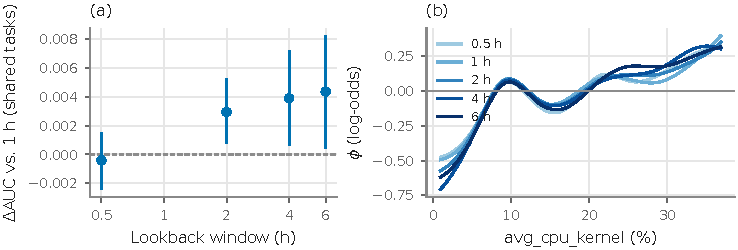
\includegraphics[width=0.85\linewidth]{figures/lookback.pdf}
\caption{Lookback ablation on the original sample. (a) AUC of each window minus the one-hour model on the test tasks both score, with paired 95\% intervals. (b) The \feat{avg_cpu_kernel} curve at each window.}
\label{fig:lookback}
\end{figure}
